\documentclass[landscape]{foils}
\usepackage{graphicx}
\usepackage{amsmath}
\usepackage[pdf]{pstricks}
\input defs.tex
\raggedright
\special{! TeXDict begin /landplus90{true}store end }
\renewcommand{\oursection}[1]{
\foilhead[-1.0cm]{#1}
}

\title{An introduction to lightlabsFDS}
\author{}
\MyLogo{}
\date{}

\begin{document}
\setlength{\parskip}{0cm}
\maketitle

\BIT \itemsep -1pt
\I  The lightlabsFDS mission
\I  Solver
\I  Interface
\I  Hardware
\I  End it
\EIT

\vfill


\oursection{The lightlabsFDS mission}
\textbf{To enable engineers and scientists to characterize optical structures 
        quickly, simply, and cost-effectively.}
\vspace{10 mm}

Innovate on three fronts to make this a reality:
\BIT
\I  Solve for electromagnetic fields in the frequency domain,
\I  Run simulations from pre-installed scientific software (Matlab), 
\I  Offload computation to centralized custom-tuned hardware.
\EIT

\oursection{Solving electromagnetics in the frequency domain}
\BIT
\I  lightlabsFDS: Frequency-Domain Solver
\I  Solves 
    \BEQ \nabla \times \mu^{-1} \nabla \times E - \omega^2 \epsilon E 
            = -i \omega J. \EEQ
    \BIT
    \I  Inputs: frequency $(\omega)$, structure $(\mu, \epsilon)$, 
            and excitation $(J)$.
    \I  Outputs: electromagnetic fields $(E, H, D, B)$.
    \EIT
\I  \emph{Many} practical advantages over existing time-domain solvers.
\EIT
\newpage
   
\oursection{Example}

\psset{unit=1.5cm}
\psset{gridcolor=green, subgridcolor=yellow}
\begin{center}
\begin{pspicture}(8,5)
    \let\psgrid\relax

    \psframe*[linecolor=lightgray,fillcolor=lightgray,fillstyle=solid]
        (1,2.2)(4,2.8)
    \psframe*[linecolor=lightgray,fillcolor=lightgray,fillstyle=solid]
        (3,1)(5,4)
    \psframe*[linecolor=lightgray,fillcolor=lightgray,fillstyle=solid]
        (4,1.4)(7,2)
    \psframe*[linecolor=lightgray,fillcolor=lightgray,fillstyle=solid]
        (4,3.0)(7,3.6)
    \rput[B](4,4.2){\textrm{Device}}
    \psline[linestyle=dashed](1.6,0.6)(1.6,4.0)
    \rput[B](1.6,4.2){\textrm{in}}
    \psline[linestyle=dashed](6.4,0.6)(6.4,4.0)
    \rput[B](6.4,4.2){\textrm{out}}
\end{pspicture}
\end{center}
Time-domain issues include
\BIT
\I  Input: clean excitation at input requires an auxiliary simulation
\I  Device: approximations required for material dispersion
\I  Output: overlap integrals must be repeatedly calculated 
        \emph{during} the simulation
\EIT
\newpage

% \begin{center}
\begin{pspicture}(6,5)(-6,0)
    \psgrid

    \psframe[fillstyle=none](-1,2)(1,3)
    \rput(0,2.5){\textrm{TDS}}

    \psline(-2.4,2.5)(-1,2.5)
    \rput[B](-1.6,2.7){$x(t)$}

    \pspolygon[fillcolor=lightgray,fillstyle=solid]
        (-2.4,4)(-2.4,1)(-3.2,0.5)(-3.2,4.5)
    \psline(-4,4)(-3.2,4) \rput(-4.8,4){$X(\omega_1)$}
    \psline(-4,3)(-3.2,3) \rput(-4.8,3){$X(\omega_2)$}
    \psline(-4,2)(-3.2,2) \rput(-4.8,2){$\vdots$}
    \psline(-4,1)(-3.2,1) \rput(-4.8,1){$X(\omega_n)$}

    \psline(2.4,2.5)(1,2.5)
    \rput[B](1.6,2.7){$y(t)$}

    \pspolygon[fillcolor=lightgray,fillstyle=solid]
        (2.4,4)(2.4,1)(3.2,0.5)(3.2,4.5)
    \psline(4,4)(3.2,4) \rput(4.8,4){$Y(\omega_1)$}
    \psline(4,3)(3.2,3) \rput(4.8,3){$Y(\omega_2)$}
    \psline(4,2)(3.2,2) \rput(4.8,2){$\vdots$}
    \psline(4,1)(3.2,1) \rput(4.8,1){$Y(\omega_n)$}
\end{pspicture}
% \end{center}
\BIT
\I  Fundamental problem: trying to use a time-domain solver as a 
        frequency-domain solver.
\I  Additionally, no method to measure simulation error!
\EIT
\newpage

\begin{center}
\begin{pspicture}(6,4)(-6,-2)
    \psgrid

    \psframe[fillstyle=none](-1,2)(1,3)
    \rput(0,2.5){\textrm{FDS}}
    \psline(-2.4,2.5)(-1,2.5)
    \rput(-3.2,2.5){$X(\omega_1)$}
    \psline(2.4,2.5)(1,2.5)
    \rput(3.2,2.5){$Y(\omega_1)$}

    \psframe[fillstyle=none](-1,0.6)(1,1.6)
    \rput(0,1.1){\textrm{FDS}}
    \psline(-2.4,1.1)(-1,1.1)
    \rput(-3.2,1.1){$X(\omega_2)$}
    \psline(2.4,1.1)(1,1.1)
    \rput(3.2,1.1){$Y(\omega_2)$}

    \rput(0,0.2){$\vdots$}

    \psframe[fillstyle=none](-1,-0.4)(1,-1.4)
    \rput(0,-0.9){\textrm{FDS}}
    \psline(-2.4,-0.9)(-1,-0.9)
    \rput(-3.2,-0.9){$X(\omega_n)$}
    \psline(2.4,-0.9)(1,-0.9)
    \rput(3.2,-0.9){$Y(\omega_n)$}
\end{pspicture}
\end{center}
\BIT
\I  Allow direct access to frequency-domain data.
\I  Take care of input and output fields outside of the simulation.
\I  Material dispersion explicitly defined.
\I  Simulation error well defined.
\EIT
\newpage

\begin{center}
% 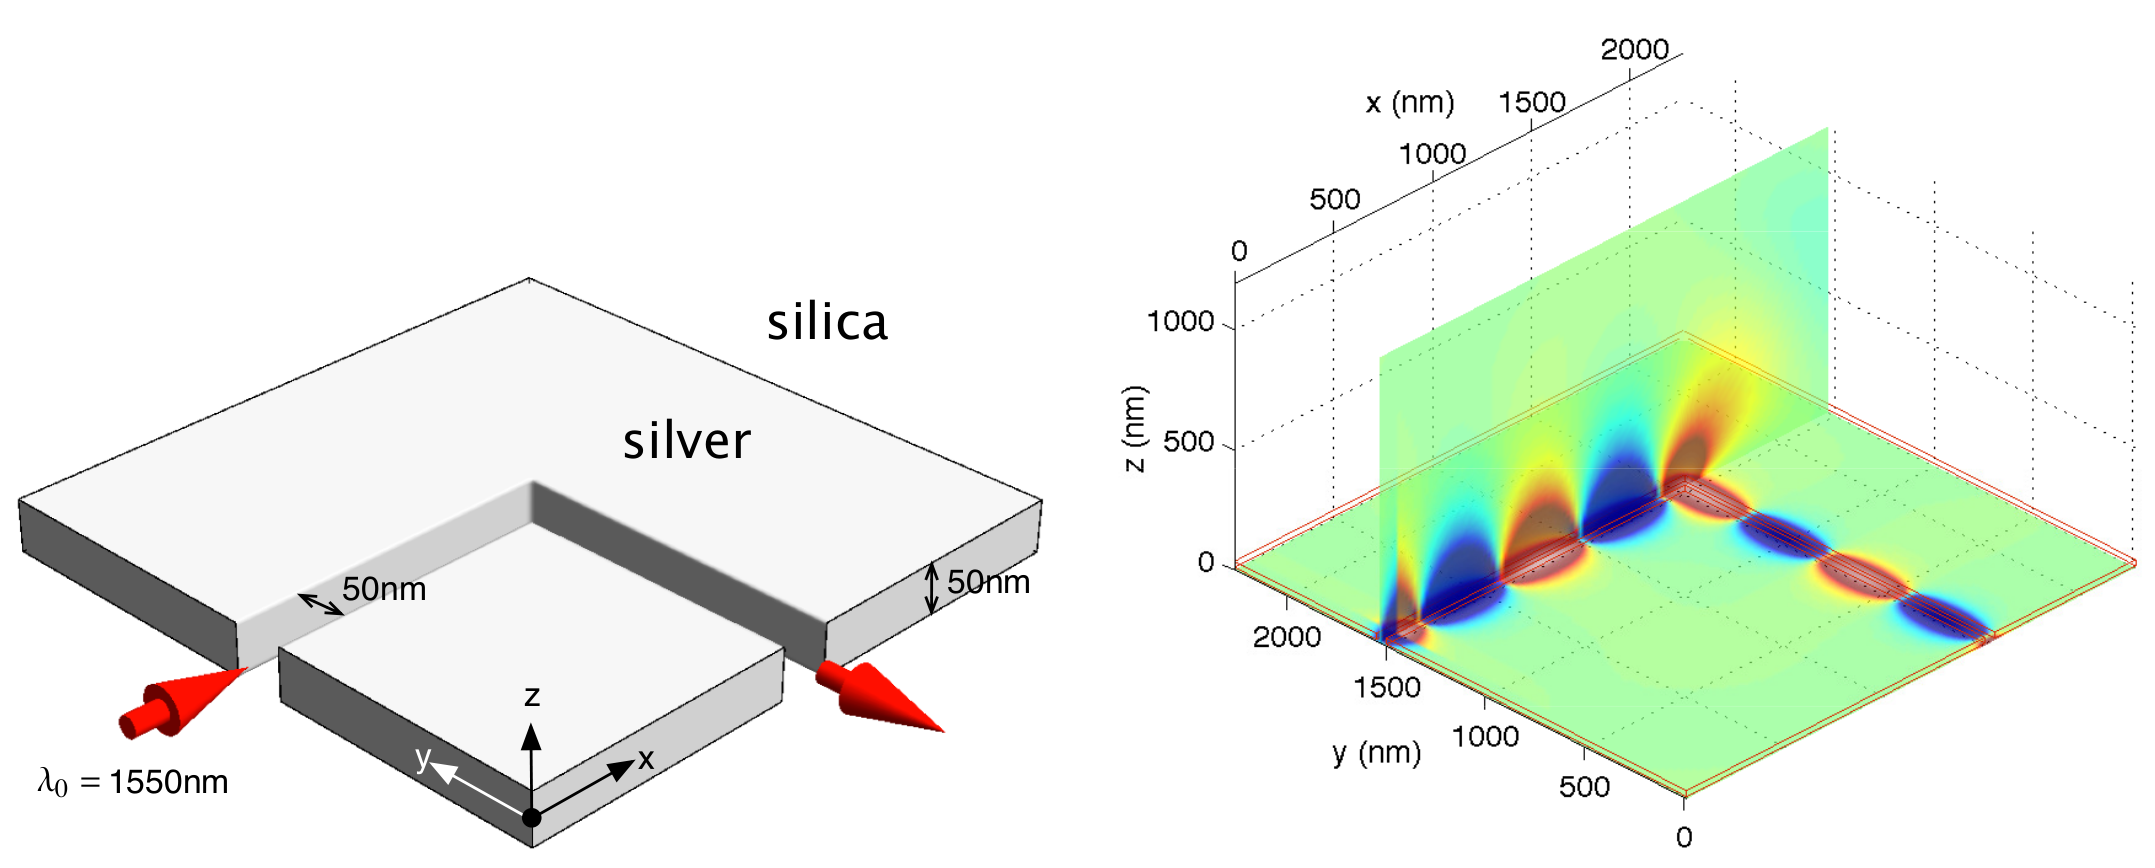
\includegraphics[width=\textwidth]{pml_cutout}
\end{center}
\BIT
\I  Frequency-domain solver made possible by correct choice of PML and 
        linear algebra algorithm.
\I  See: Wonseok Shin, Shanhui Fan, 
            ``Choice of the perfectly matched layer boundary condition for 
            frequency-domain Maxwell's equations solvers'',
            Journal of Computational Physics (January 2012).
\EIT


\oursection{Interface}
\textbf{We want engineers and scientists to absolutely love using FDS
        and, at the same time, to forget about it because it just works.}
\BIT
\I  No installation, just start up Matlab and
\begin{verbatim}
>>> [E, H] = fds(omega, epsilon, J); % Done.
\end{verbatim}
\I  Helper functions to
    \BIT
    \I  construct the optical structures $(\epsilon, \mu)$,
    \I  define the input excitations $(J)$, and
    \I  analyze and visualize the output fields $(E,H,D,B)$
    \EIT
    are all included and open-sourced.
\I  Additionally, lots of examples and tutorials.
\EIT

\oursection{Hardware}
\begin{center}
\begin{pspicture}(6,3)(-6,-3)
    \psgrid
    \rput(0,0){\parbox{5cm}{\begin{center}\textrm{lightlabsFDS\\server}
                            \end{center}}}
    \psline{<->}(-1.2,0.8)(-2.8,1.4) \rput(-3.5,1.5){\textrm{user1}}
    \psline{<->}(-3.2,0)(-1.6,0) \rput(-4,0){\textrm{user2}}
    \psline{<->}(-1.2,-0.8)(-2.8,-1.4) \rput(-3.5,-1.5){\textrm{user3}}
    \psline{<->}(1.2,0.8)(2.8,1.4) \rput(3.5,1.5){\textrm{user4}}
    \psline{<->}(3.2,0)(1.6,0) \rput(4,0){$\vdots$}
    \psline{<->}(1.2,-0.8)(2.8,-1.4) \rput(3.5,-1.5){\textrm{userN}}
\end{pspicture}
\end{center}
\BIT
\I  Centralized, shared, custom-tuned server able to deliver the performance
        of a large cluster
\I  Performance achieved via heavily optimized GPU code
\I  Multiple servers can be clustered with nearly $100\%$ computational
        efficiency.
\EIT

\oursection{Current status}
\BIT
\I  Algorithm: Implemented on GPUs, still optimizing (Jesse)
\I  Interface: (Wonseok)
\I  Hardware: Prototype ordered and being built (Jesse)
\EIT
\end{document}
